\chapter*{Appendix}
\renewcommand{\thefigure}{A.\arabic{figure}}
\setcounter{figure}{0}  
\section*{One-stage Experiment Results}
\begin{figure}[H]
  \caption{Optimization using dynamic friction}
  \begin{subfigure}[t]{0.5\textwidth}
    \centering
    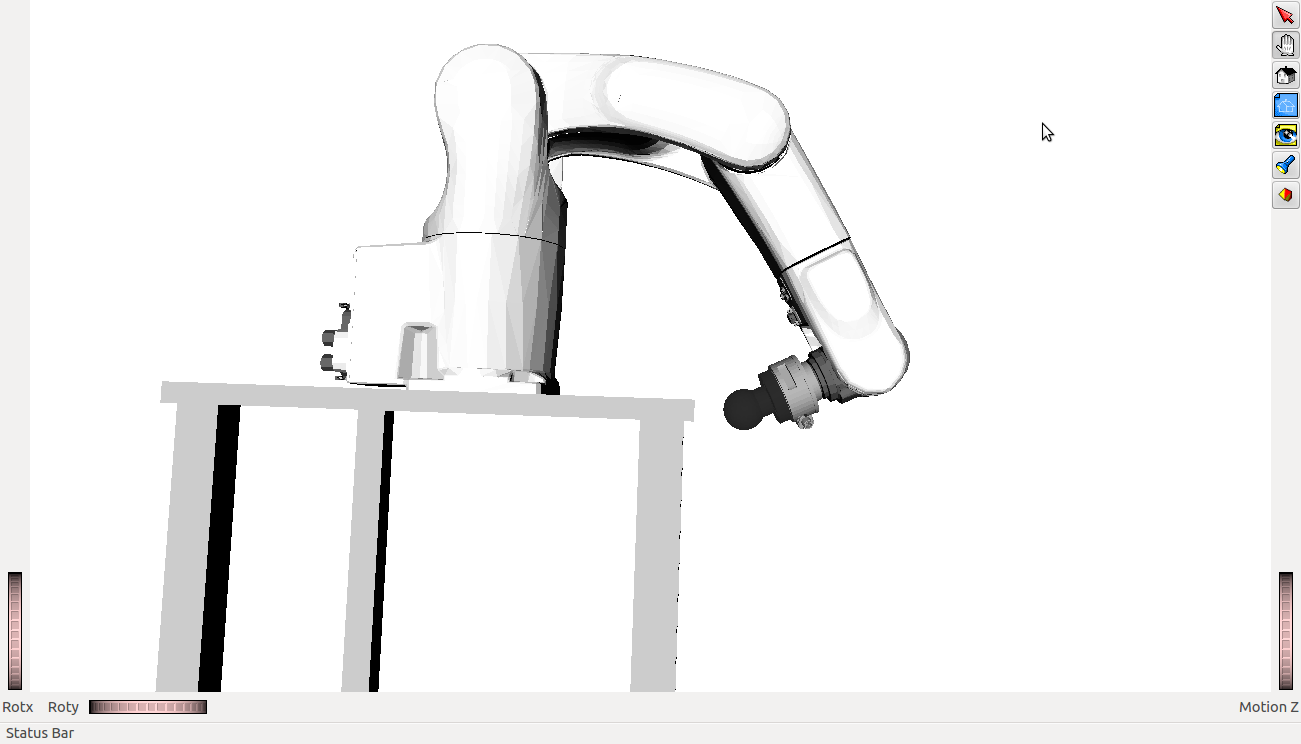
\includegraphics[width = \textwidth ]{one_stage_1} 
    \caption{First Joint}
  \end{subfigure}
  \begin{subfigure}[t]{0.5\textwidth}
    \centering
    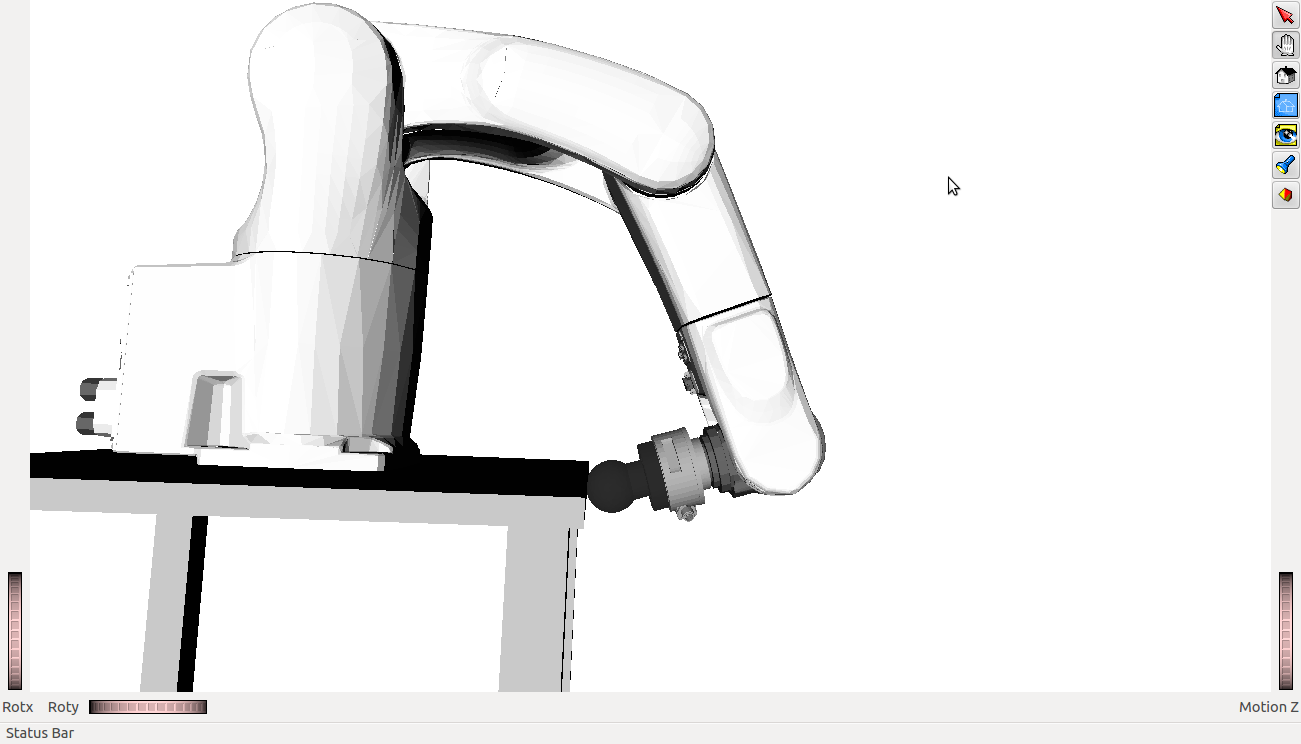
\includegraphics[width = \textwidth ]{one_stage_2}
    \caption{Second Joint}
  \end{subfigure}
  \begin{subfigure}[t]{0.5\textwidth}
    \centering
    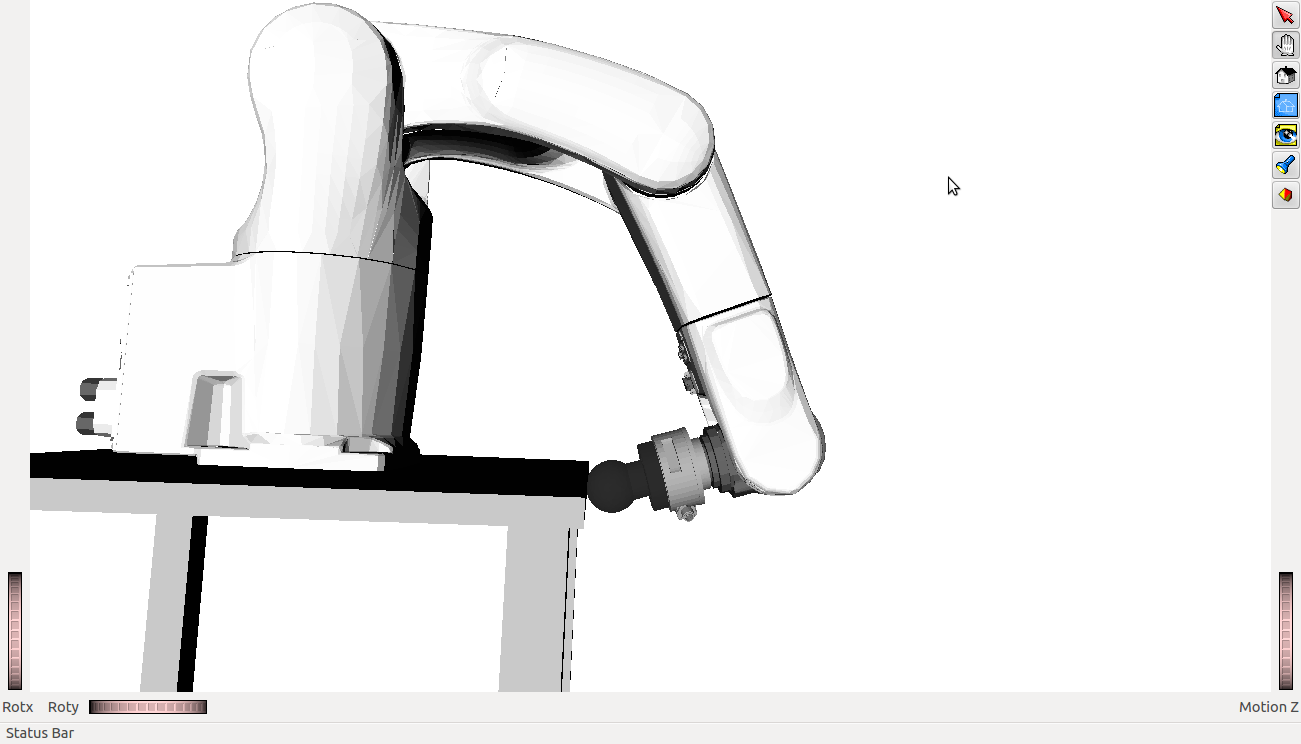
\includegraphics[width = \textwidth ]{one_stage_2}
    \caption{Third Joint}
  \end{subfigure}
  \begin{subfigure}[t]{0.5\textwidth}
    \centering
    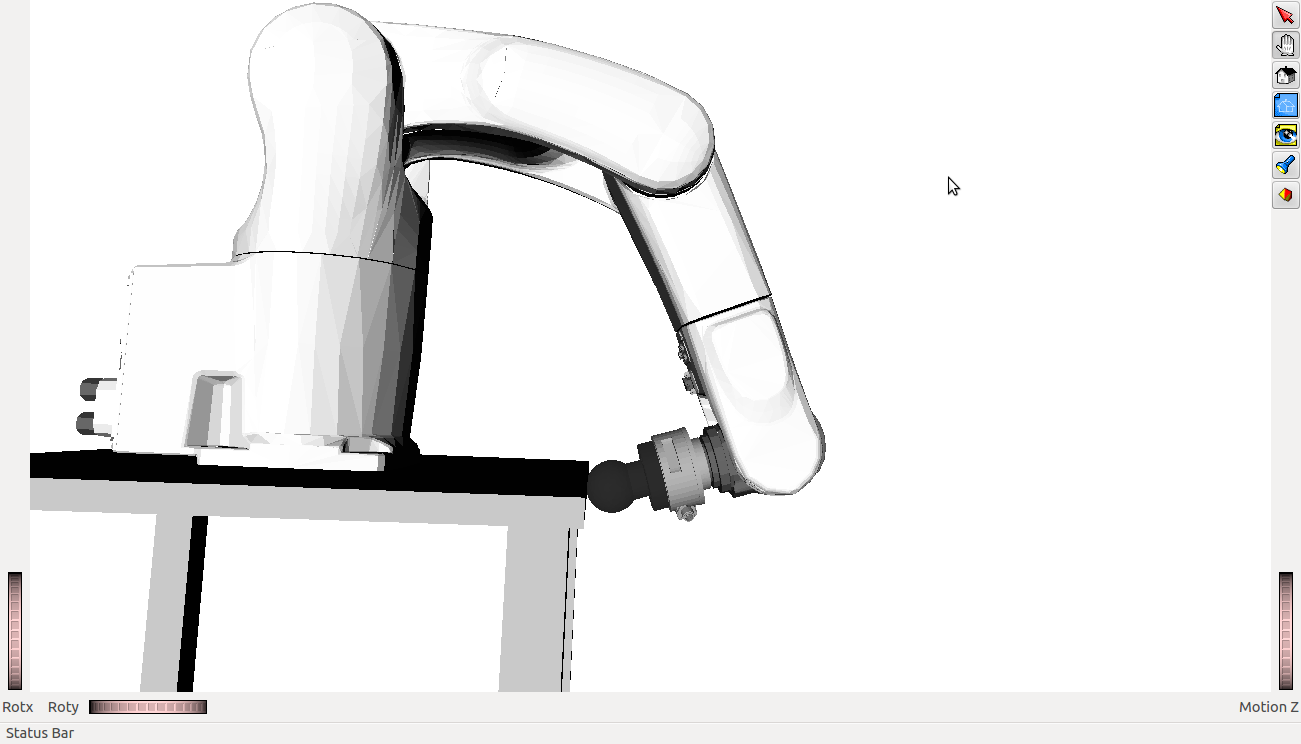
\includegraphics[width = \textwidth ]{one_stage_2}
    \caption{Fourth Joint}
  \end{subfigure}
  \begin{subfigure}[t]{0.5\textwidth}
    \centering
    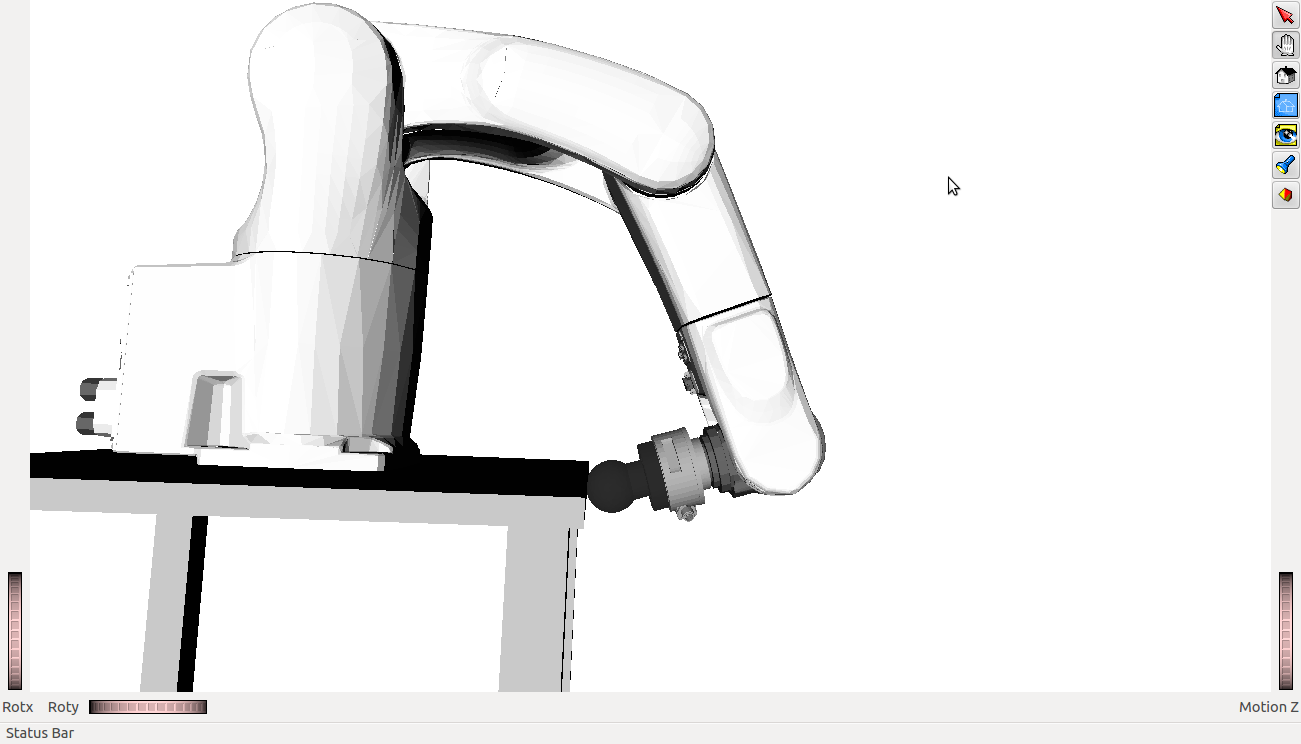
\includegraphics[width = \textwidth ]{one_stage_2}
    \caption{Fifth Joint}
  \end{subfigure}
  \begin{subfigure}[t]{0.5\textwidth}
    \centering
    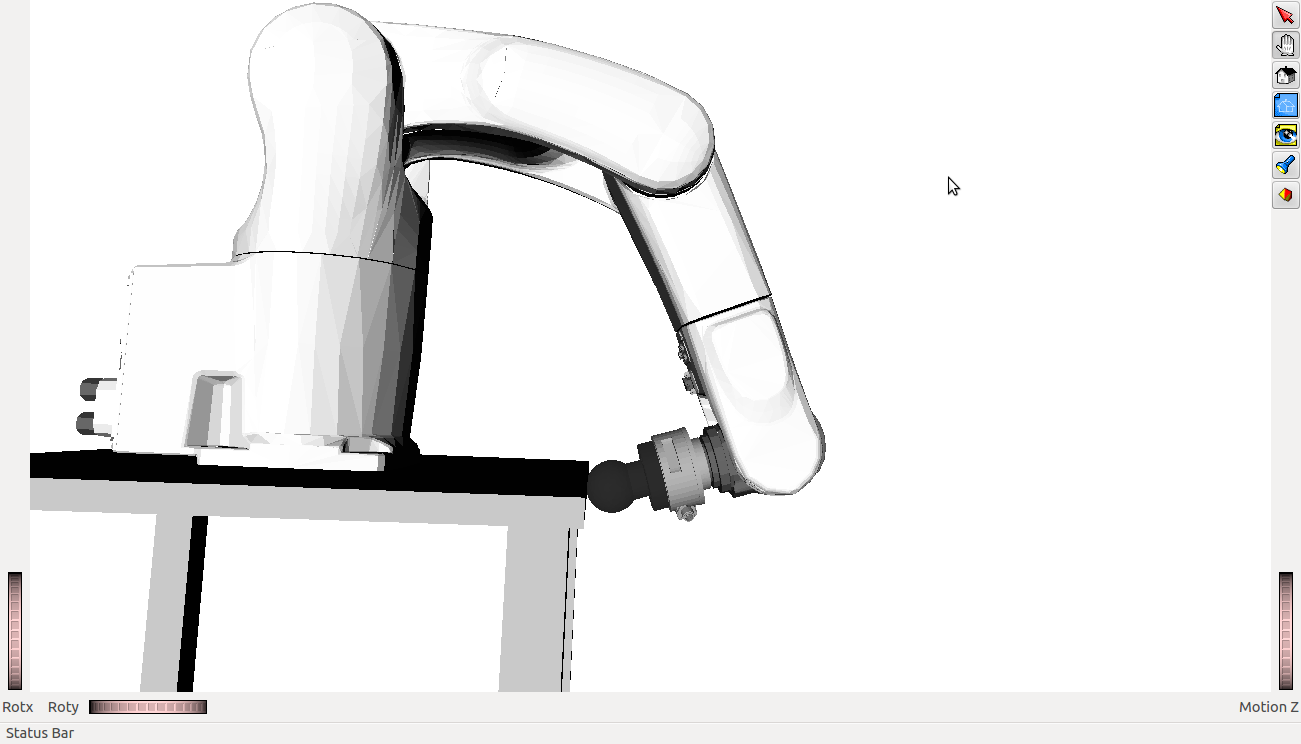
\includegraphics[width = \textwidth ]{one_stage_2}
    \caption{Sixth Joint}
  \end{subfigure}
\end{figure}

\begin{figure}[H]
  \caption{ptimization using static friction}
  \begin{subfigure}[t]{0.5\textwidth}
    \centering
    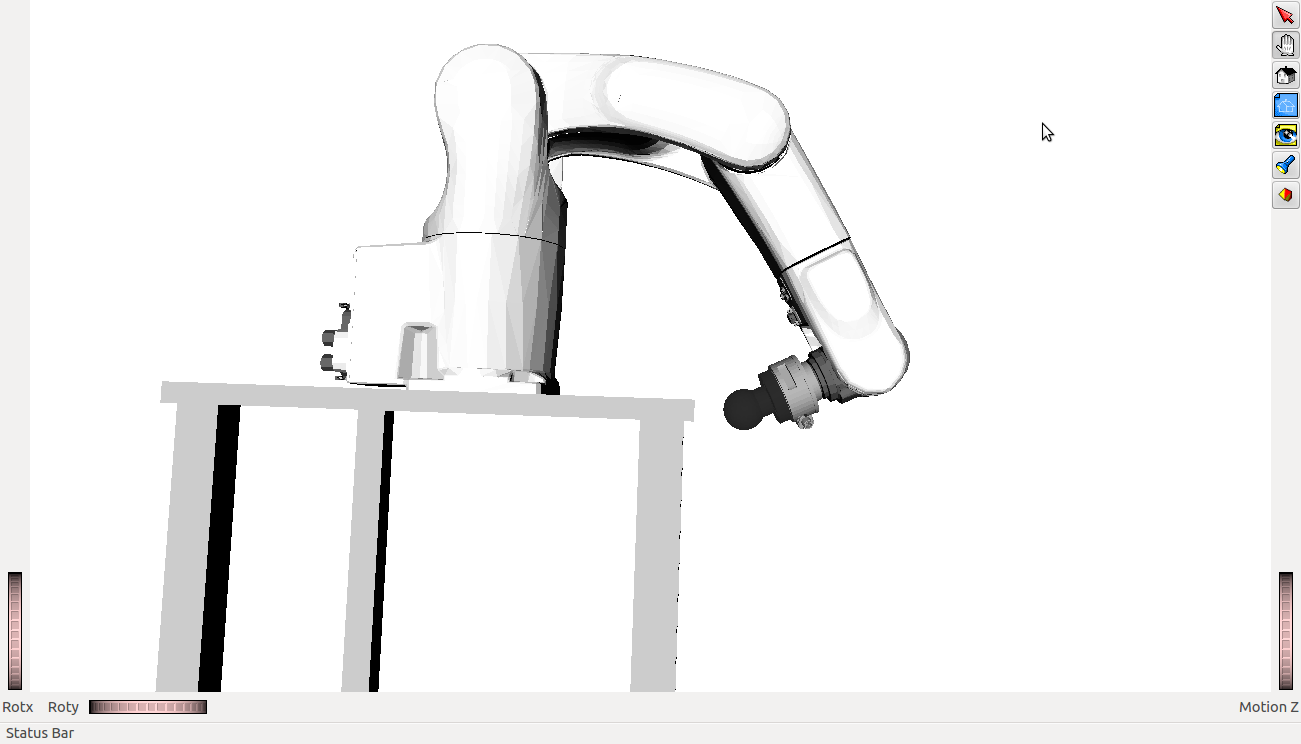
\includegraphics[width = \textwidth ]{one_stage_1} 
    \caption{First Joint}
  \end{subfigure}
  \begin{subfigure}[t]{0.5\textwidth}
    \centering
    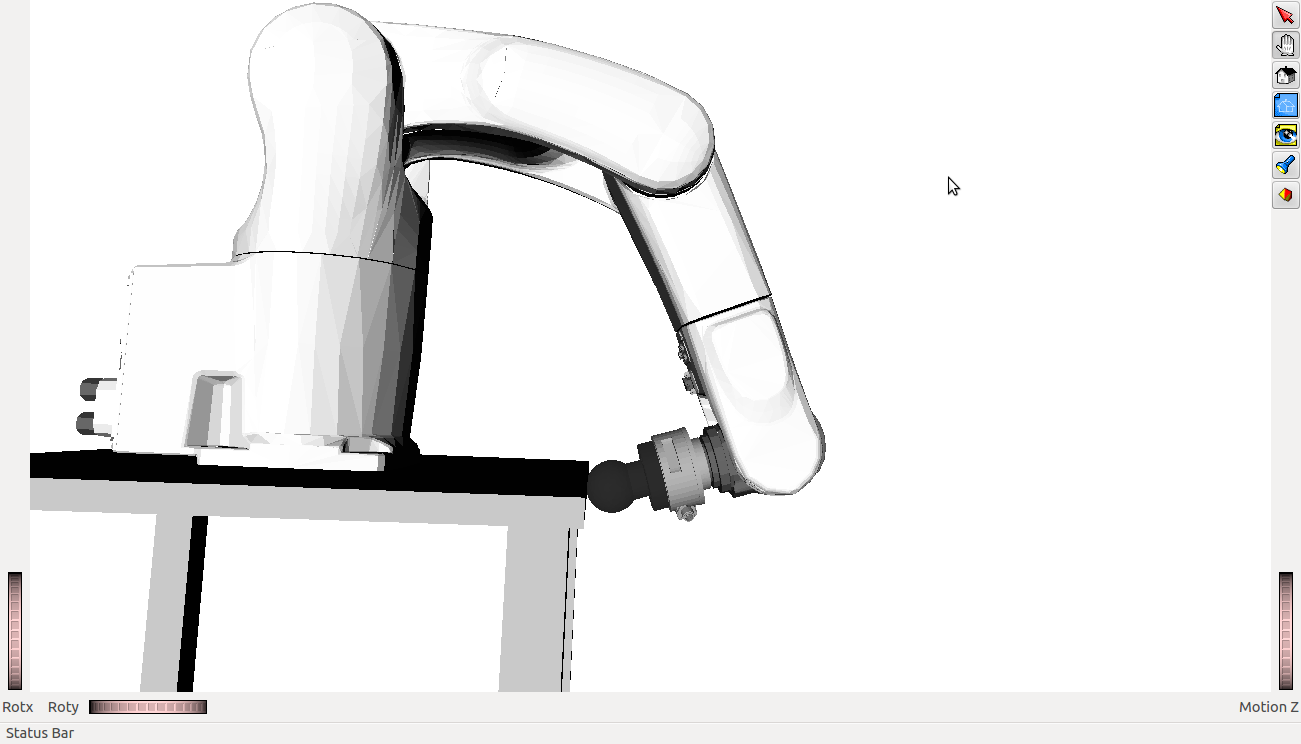
\includegraphics[width = \textwidth ]{one_stage_2}
    \caption{Second Joint}
  \end{subfigure}
  \begin{subfigure}[t]{0.5\textwidth}
    \centering
    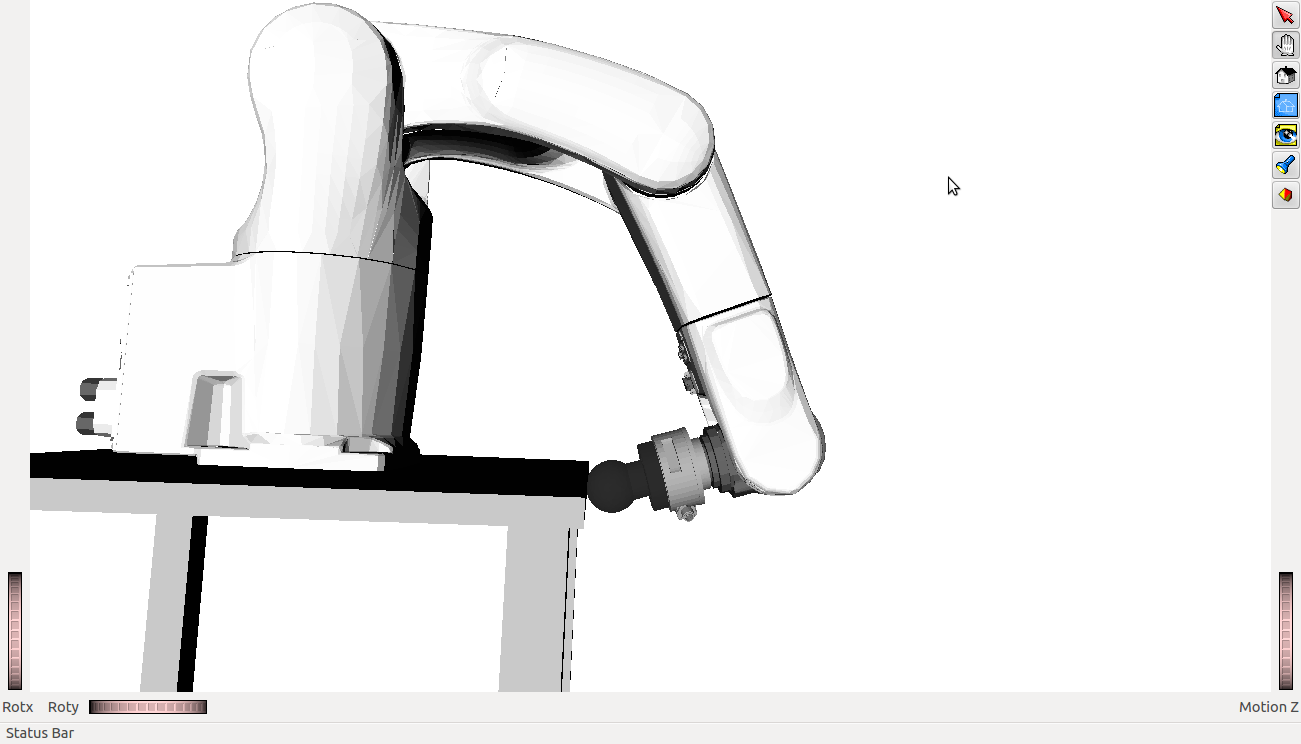
\includegraphics[width = \textwidth ]{one_stage_2}
    \caption{Third Joint}
  \end{subfigure}
  \begin{subfigure}[t]{0.5\textwidth}
    \centering
    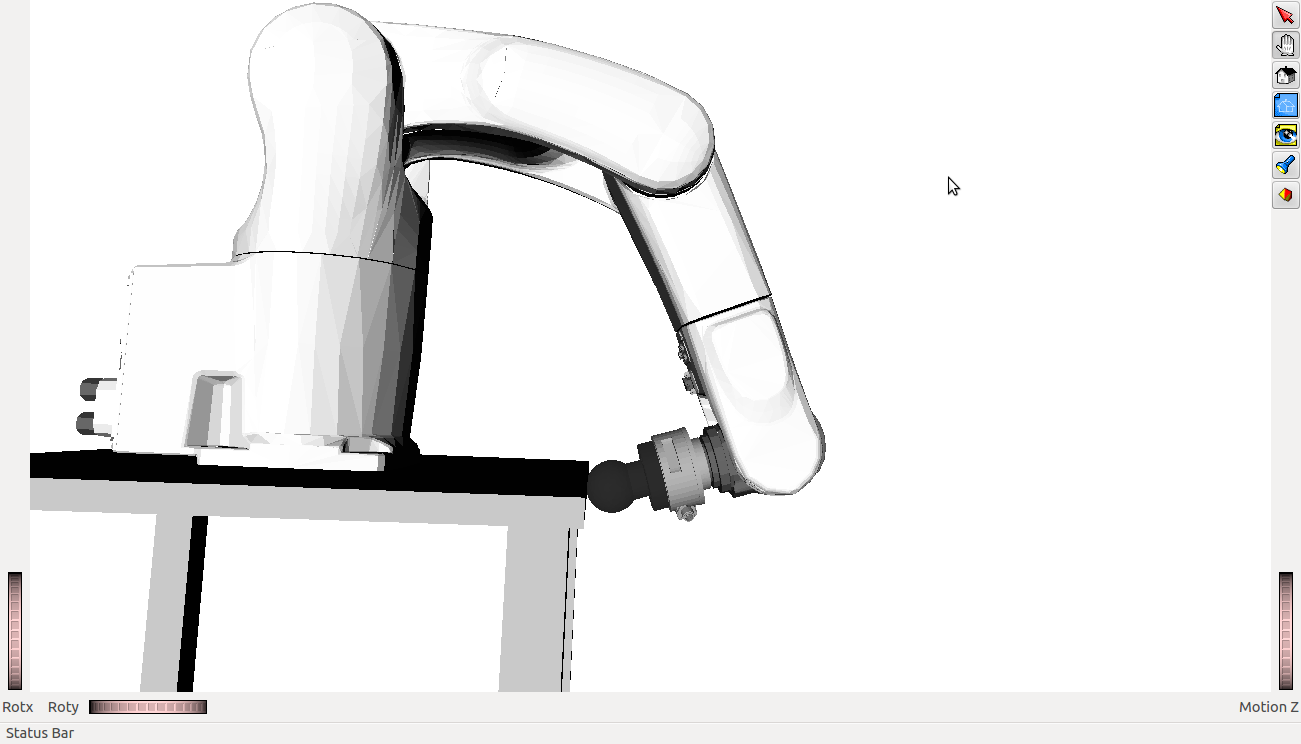
\includegraphics[width = \textwidth ]{one_stage_2}
    \caption{Fourth Joint}
  \end{subfigure}
  \begin{subfigure}[t]{0.5\textwidth}
    \centering
    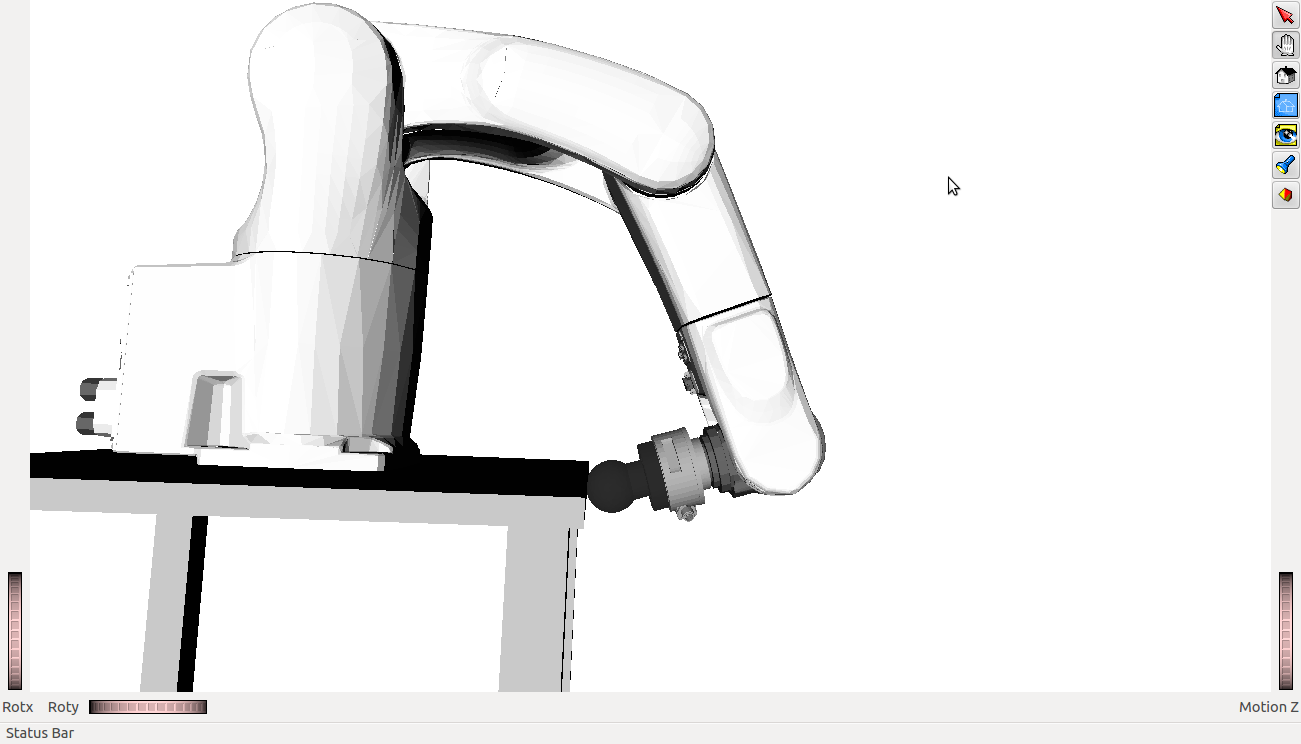
\includegraphics[width = \textwidth ]{one_stage_2}
    \caption{Fifth Joint}
  \end{subfigure}
  \begin{subfigure}[t]{0.5\textwidth}
    \centering
    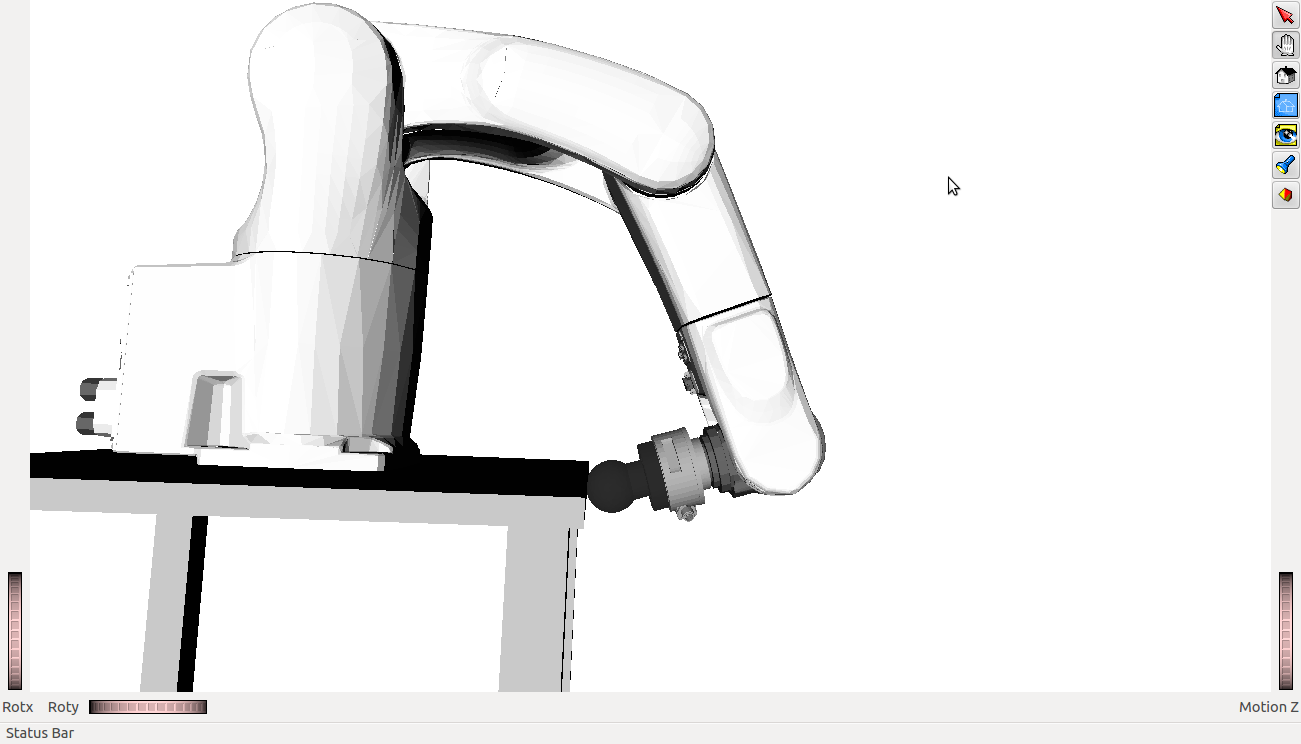
\includegraphics[width = \textwidth ]{one_stage_2}
    \caption{Sixth Joint}
  \end{subfigure}
\end{figure}


\section*{Two-stage Experiment Results}
\subsection*{High torque Collection Data}
\begin{figure}[H]
  \caption{Denso torque during high torque experiment}
  \begin{subfigure}[t]{0.5\textwidth}
    \centering
    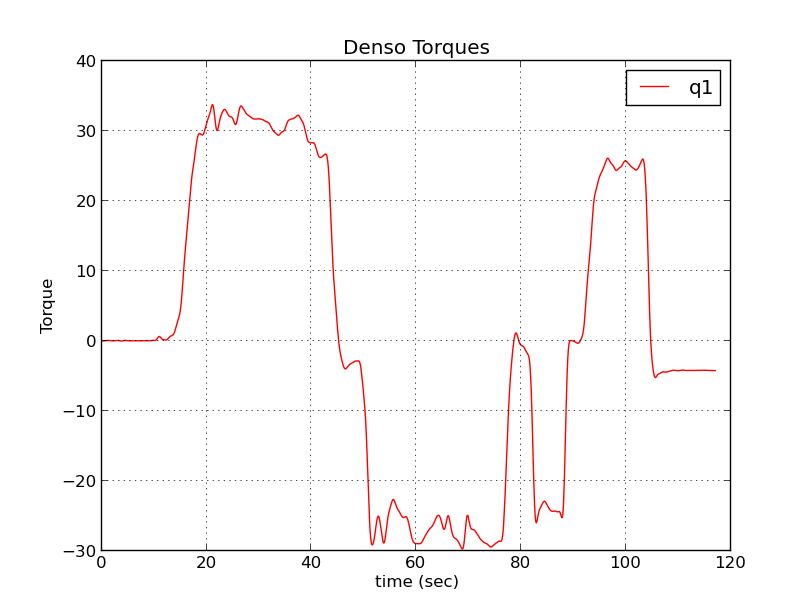
\includegraphics[width = \textwidth ]{A_4_1} 
    \caption{First Joint}
  \end{subfigure}
  \begin{subfigure}[t]{0.5\textwidth}
    \centering
    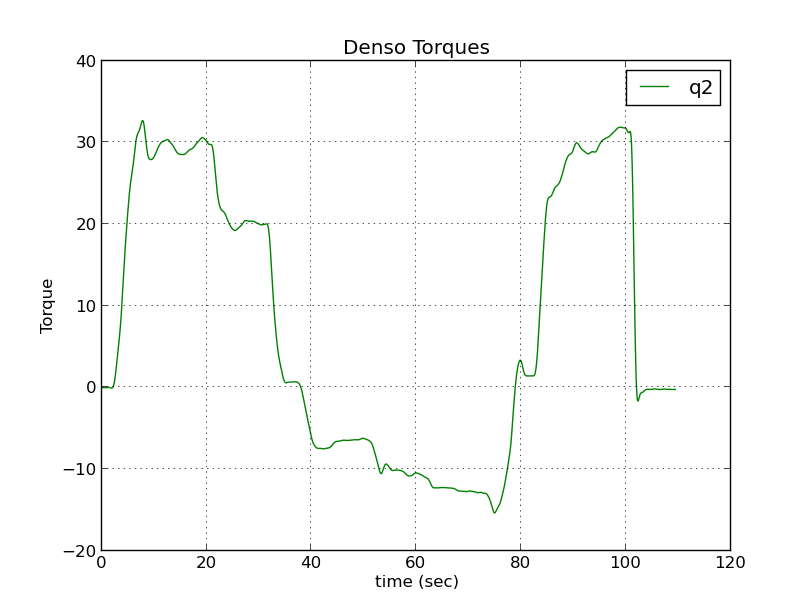
\includegraphics[width = \textwidth ]{A_4_2}
    \caption{Second Joint}
  \end{subfigure}
  \begin{subfigure}[t]{0.5\textwidth}
    \centering
    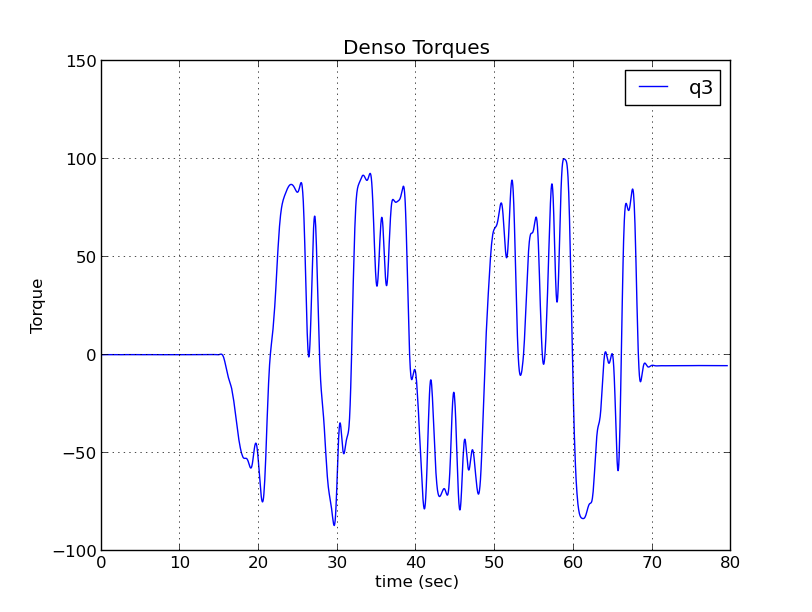
\includegraphics[width = \textwidth ]{A_4_3}
    \caption{Third Joint}
  \end{subfigure}
  \begin{subfigure}[t]{0.5\textwidth}
    \centering
    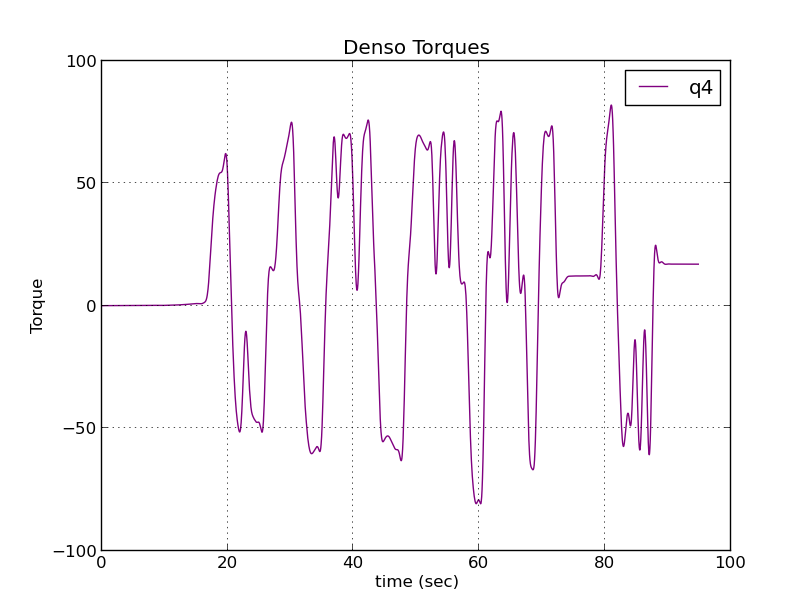
\includegraphics[width = \textwidth ]{A_4_4}
    \caption{Fourth Joint}
  \end{subfigure}
  \begin{subfigure}[t]{0.5\textwidth}
    \centering
    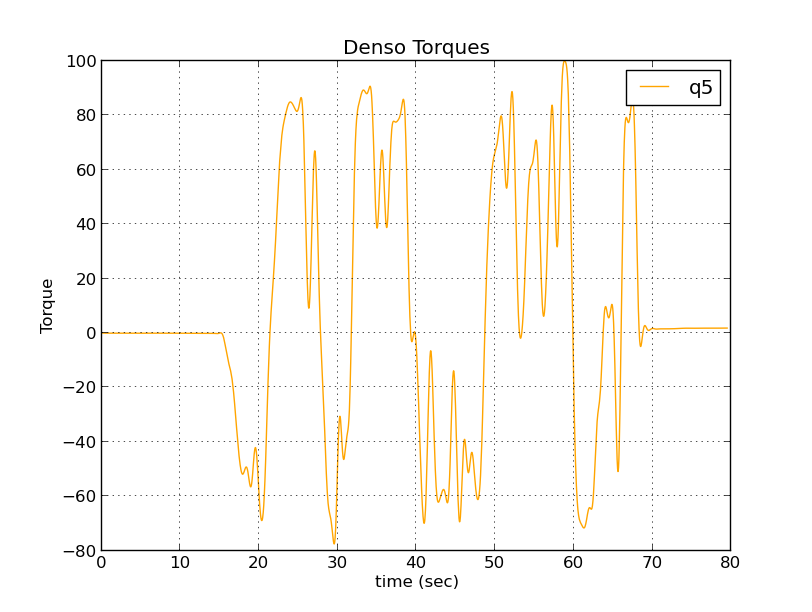
\includegraphics[width = \textwidth ]{A_4_5}
    \caption{Fifth Joint}
  \end{subfigure}
  \begin{subfigure}[t]{0.5\textwidth}
    \centering
    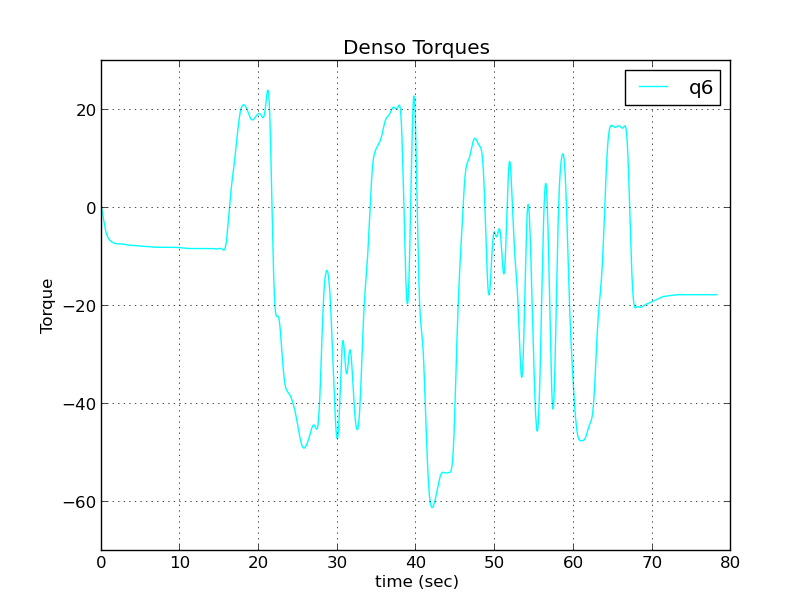
\includegraphics[width = \textwidth ]{A_4_6}
    \caption{Sixth Joint}
  \end{subfigure}
\end{figure}

\begin{figure}[H]
  \caption{External wrench during high torque experiment}
  \begin{subfigure}[t]{0.5\textwidth}
    \centering
    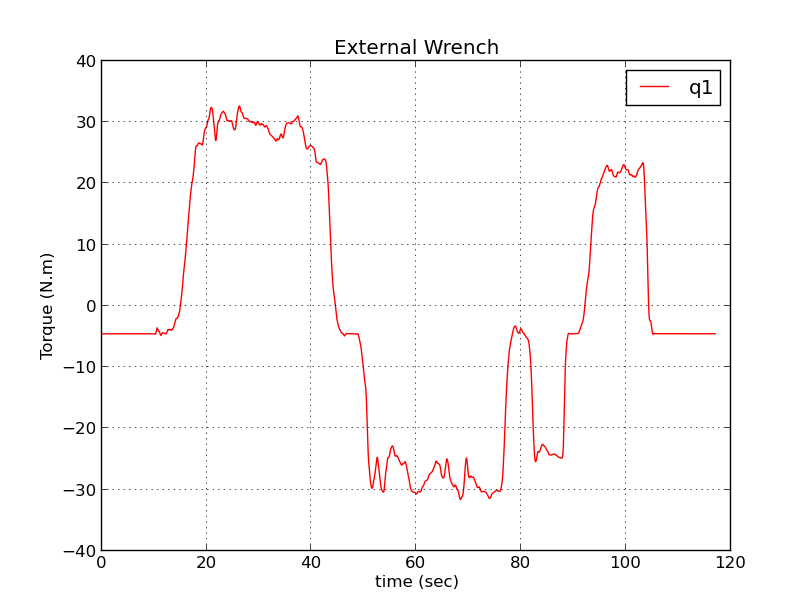
\includegraphics[width = \textwidth ]{A_5_1} 
    \caption{First Joint}
  \end{subfigure}
  \begin{subfigure}[t]{0.5\textwidth}
    \centering
    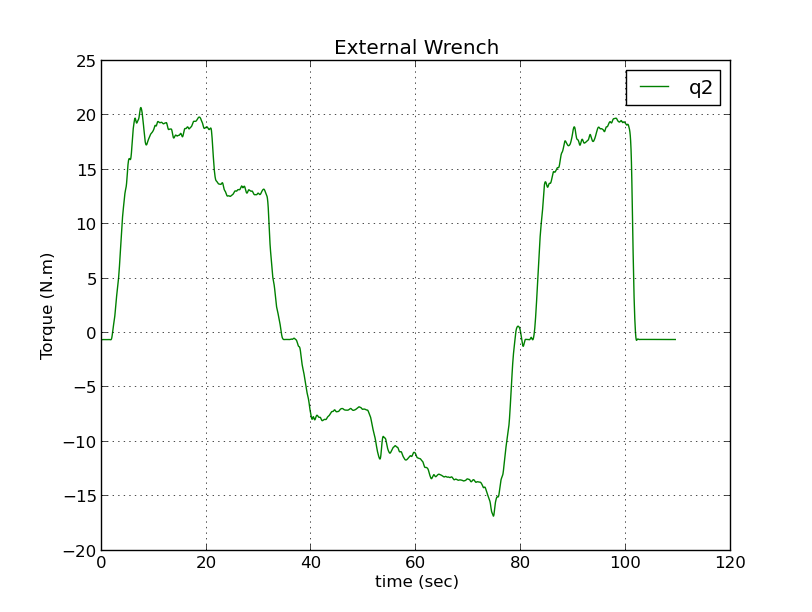
\includegraphics[width = \textwidth ]{A_5_2}
    \caption{Second Joint}
  \end{subfigure}
  \begin{subfigure}[t]{0.5\textwidth}
    \centering
    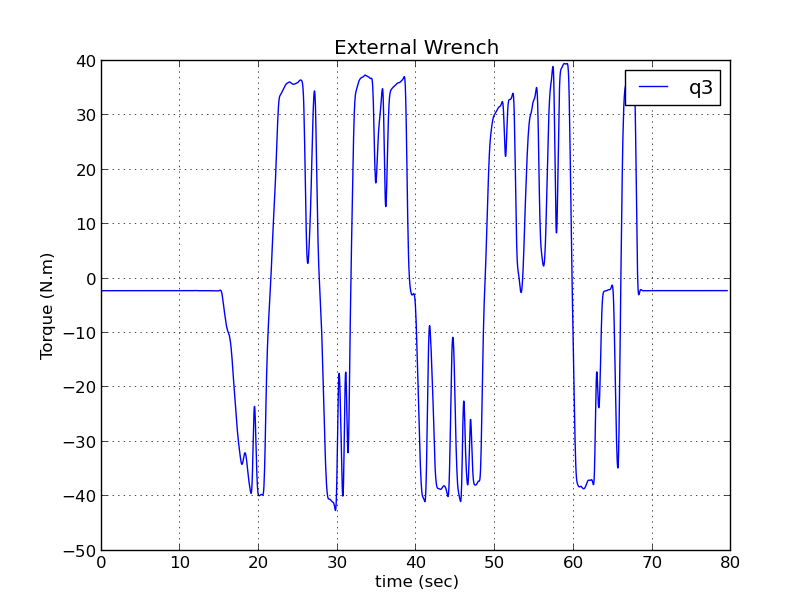
\includegraphics[width = \textwidth ]{A_5_3}
    \caption{Third Joint}
  \end{subfigure}
  \begin{subfigure}[t]{0.5\textwidth}
    \centering
    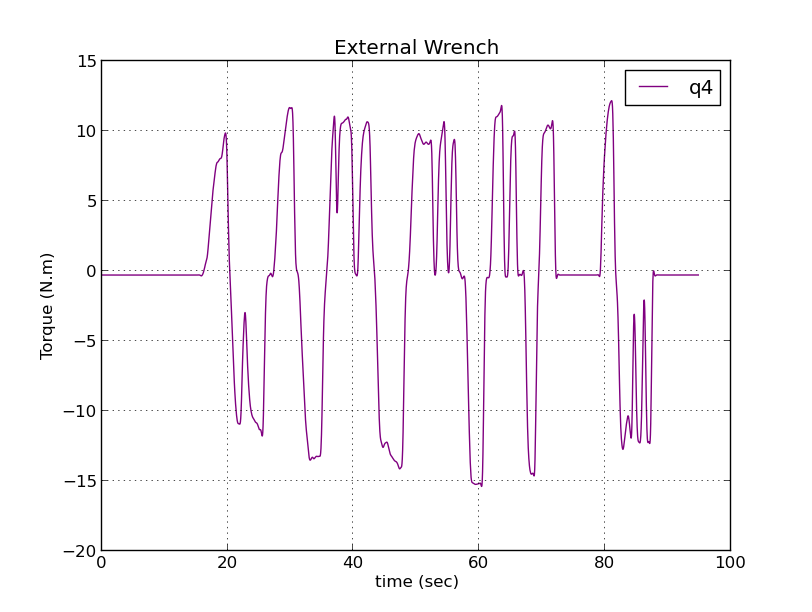
\includegraphics[width = \textwidth ]{A_5_4}
    \caption{Fourth Joint}
  \end{subfigure}
  \begin{subfigure}[t]{0.5\textwidth}
    \centering
    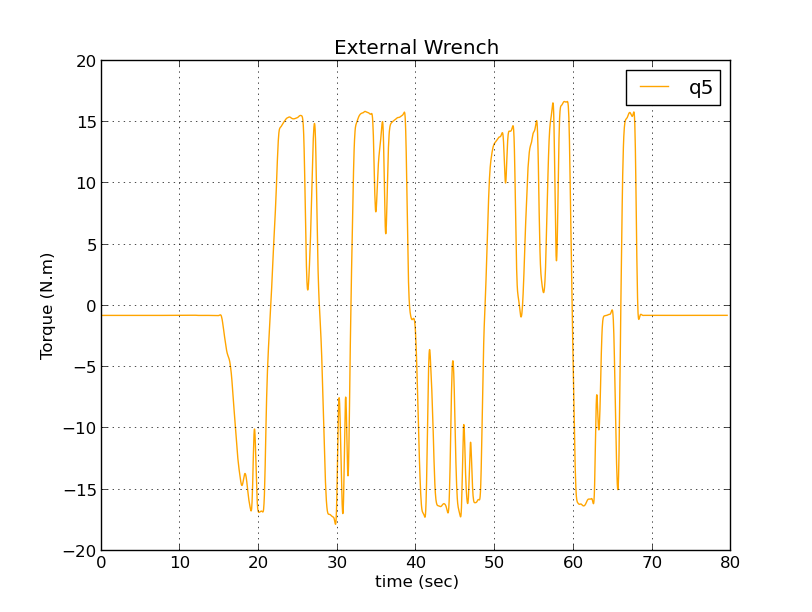
\includegraphics[width = \textwidth ]{A_5_5}
    \caption{Fifth Joint}
  \end{subfigure}
  \begin{subfigure}[t]{0.5\textwidth}
    \centering
    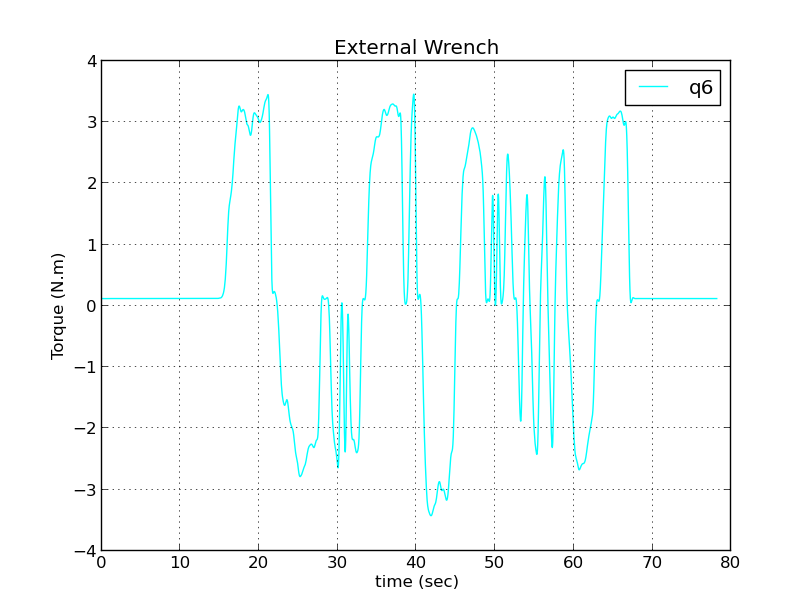
\includegraphics[width = \textwidth ]{A_5_6}
    \caption{Sixth Joint}
  \end{subfigure}
\end{figure}


\begin{figure}[H]
  \caption{Denso Gain Identification}
  \begin{subfigure}[t]{0.5\textwidth}
    \centering
    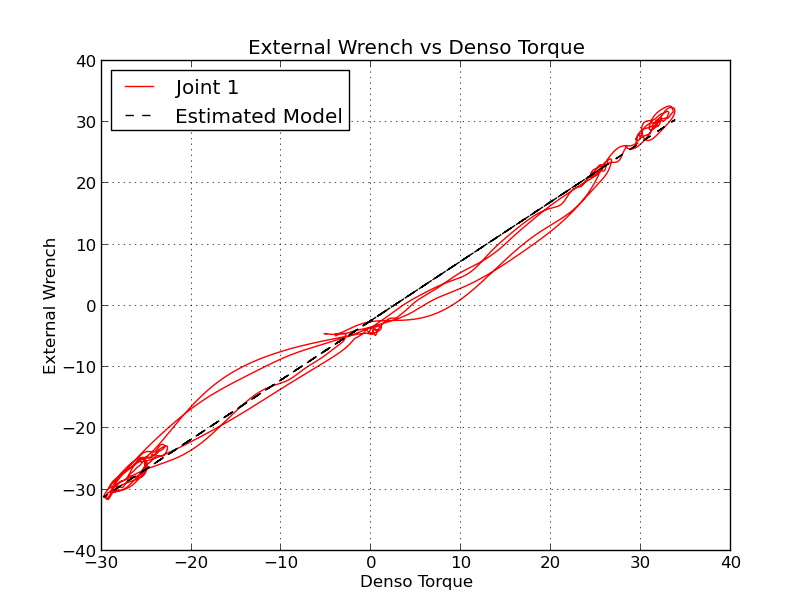
\includegraphics[width = \textwidth ]{A_6_1} 
    \caption{First Joint}
  \end{subfigure}
  \begin{subfigure}[t]{0.5\textwidth}
    \centering
    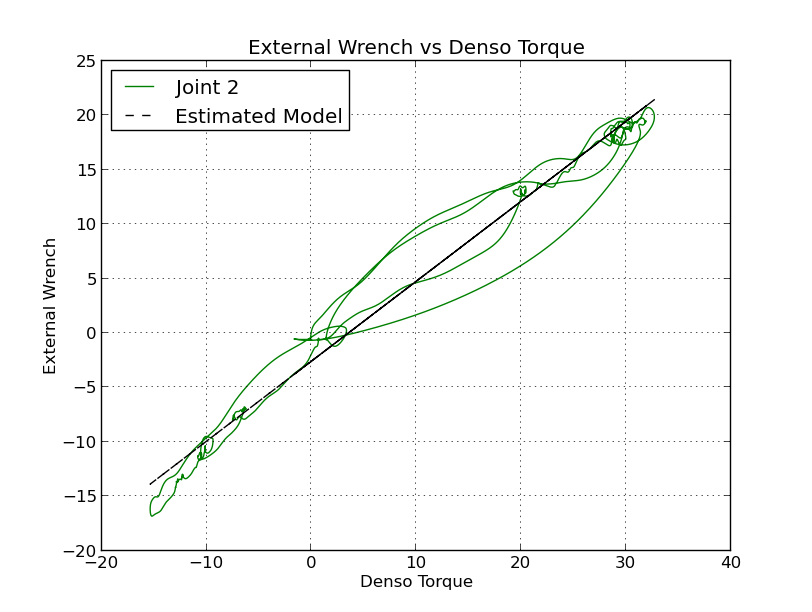
\includegraphics[width = \textwidth ]{A_6_2}
    \caption{Second Joint}
  \end{subfigure}
  \begin{subfigure}[t]{0.5\textwidth}
    \centering
    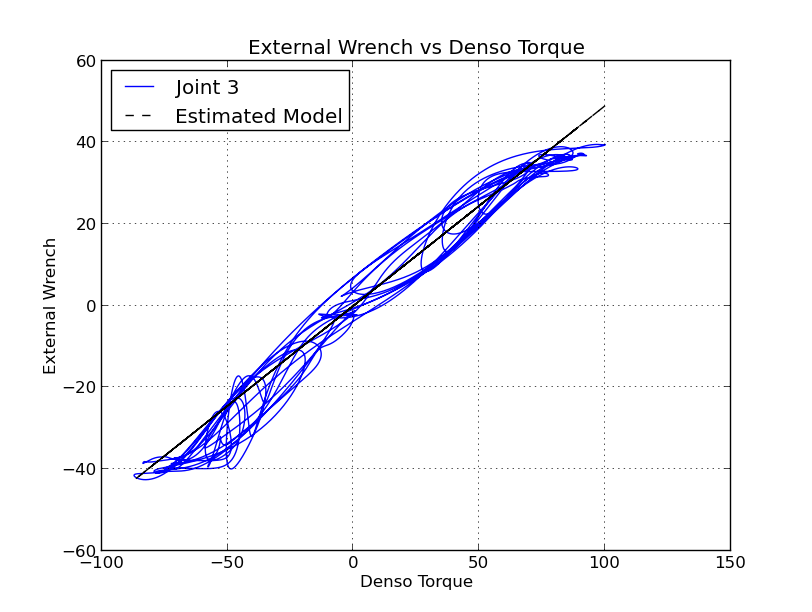
\includegraphics[width = \textwidth ]{A_6_3}
    \caption{Third Joint}
  \end{subfigure}
  \begin{subfigure}[t]{0.5\textwidth}
    \centering
    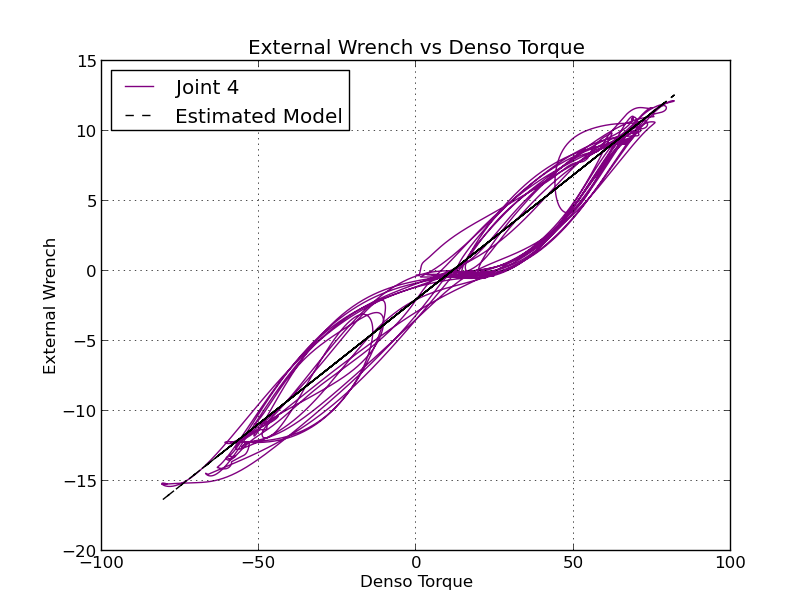
\includegraphics[width = \textwidth ]{A_6_4}
    \caption{Fourth Joint}
  \end{subfigure}
  \begin{subfigure}[t]{0.5\textwidth}
    \centering
    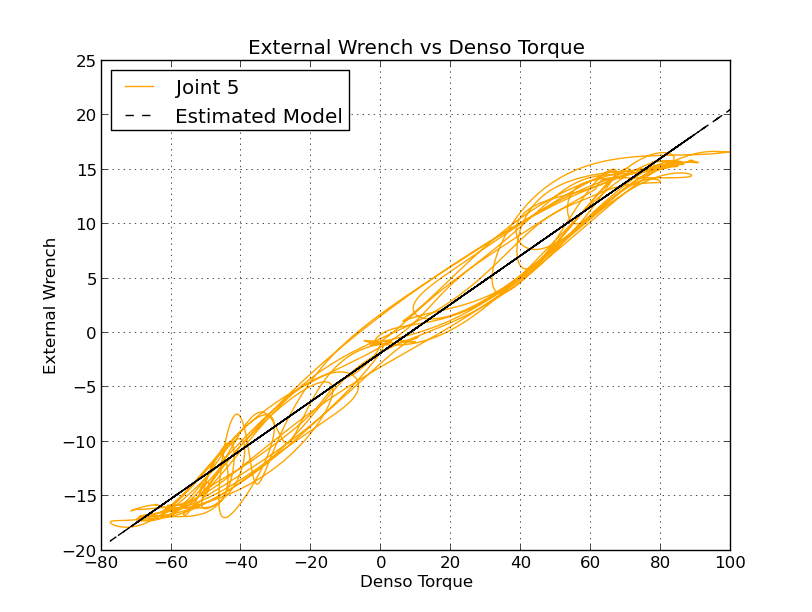
\includegraphics[width = \textwidth ]{A_6_5}
    \caption{Fifth Joint}
  \end{subfigure}
  \begin{subfigure}[t]{0.5\textwidth}
    \centering
    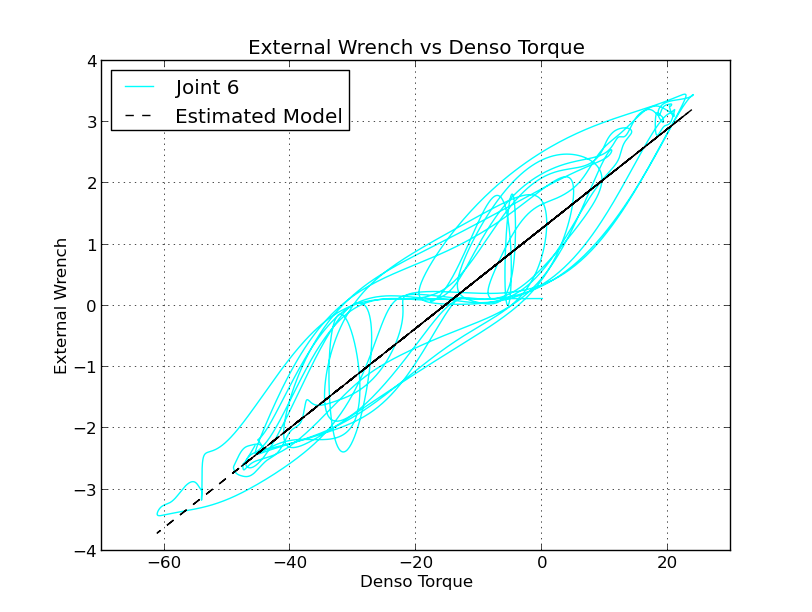
\includegraphics[width = \textwidth ]{A_6_6}
    \caption{Sixth Joint}
    \label{fig:denso gain sixth joint}
  \end{subfigure}
\end{figure}


\subsection*{High Velocity Collection Data}
\begin{figure}[H]
  \caption{Friction Identification}  
  \label{fig:appendix high vel fric}
  \begin{subfigure}[t]{0.5\textwidth}
    \centering
    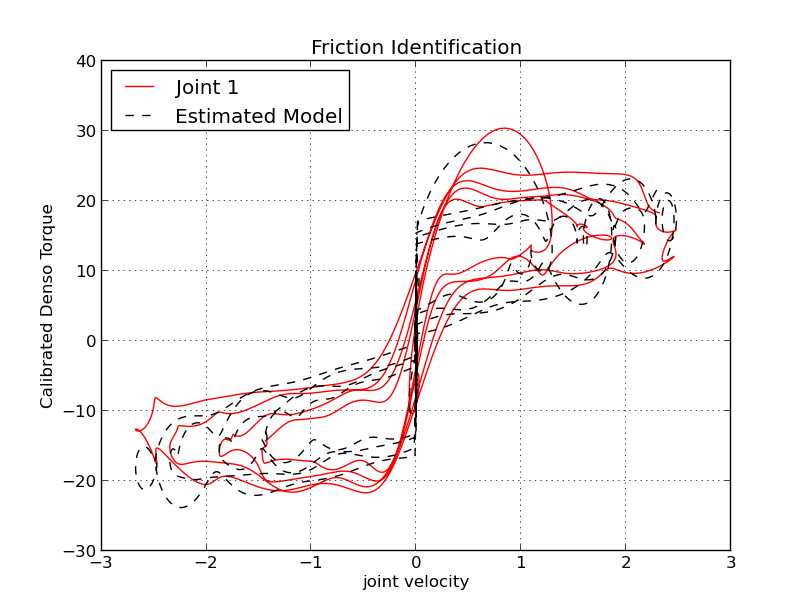
\includegraphics[width = \textwidth ]{A_7_1} 
    \caption{First Joint}
  \end{subfigure}
  \begin{subfigure}[t]{0.5\textwidth}
    \centering
    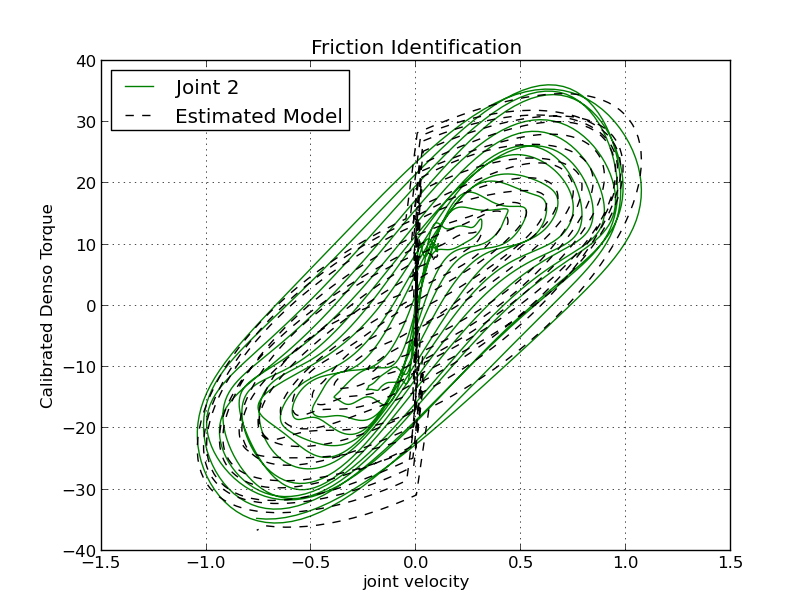
\includegraphics[width = \textwidth ]{A_7_2}
    \caption{Second Joint}
  \end{subfigure}
  \begin{subfigure}[t]{0.5\textwidth}
    \centering
    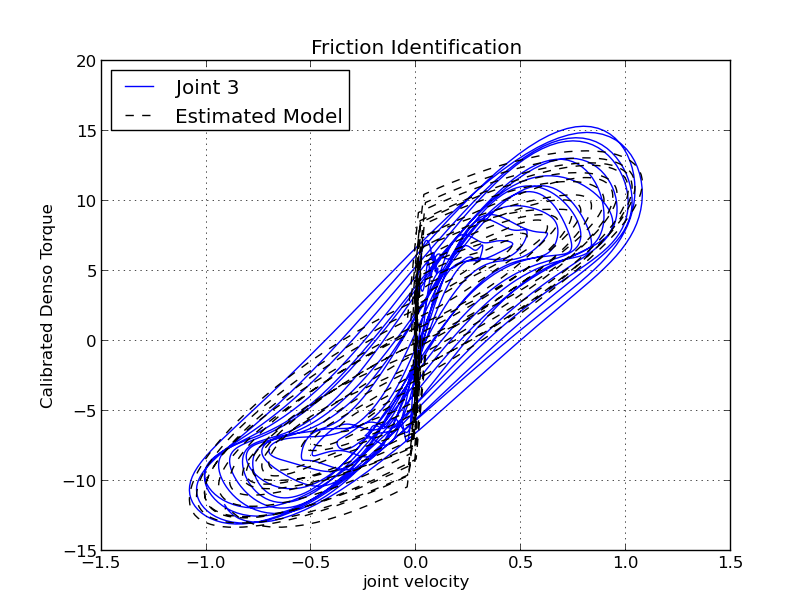
\includegraphics[width = \textwidth ]{A_7_3}
    \caption{Third Joint}
  \end{subfigure}
  \begin{subfigure}[t]{0.5\textwidth}
    \centering
    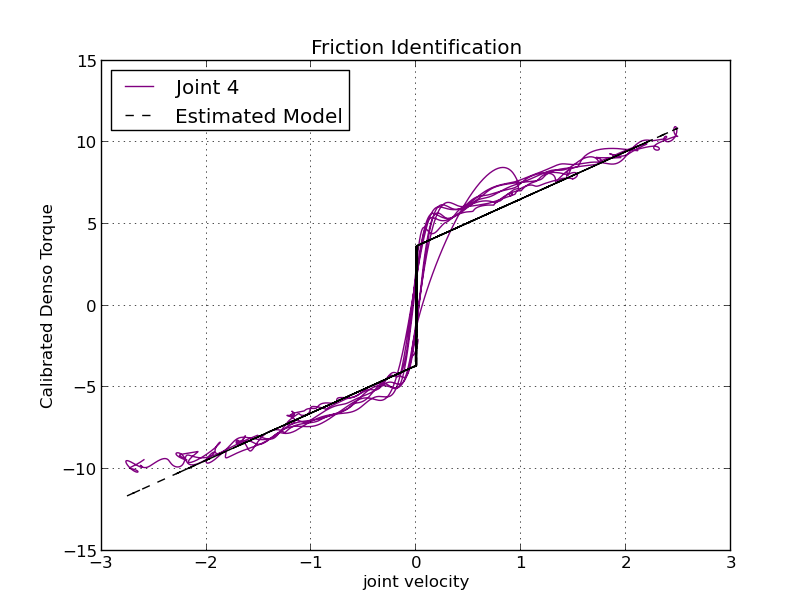
\includegraphics[width = \textwidth ]{A_7_4}
    \caption{Fourth Joint}
  \end{subfigure}
  \begin{subfigure}[t]{0.5\textwidth}
    \centering
    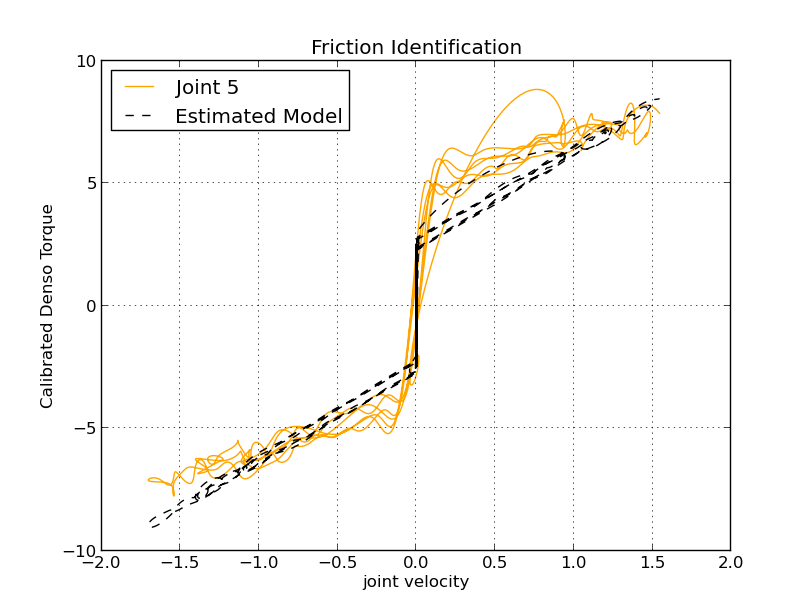
\includegraphics[width = \textwidth ]{A_7_5}
    \caption{Fifth Joint}
  \end{subfigure}
  \begin{subfigure}[t]{0.5\textwidth}
    \centering
    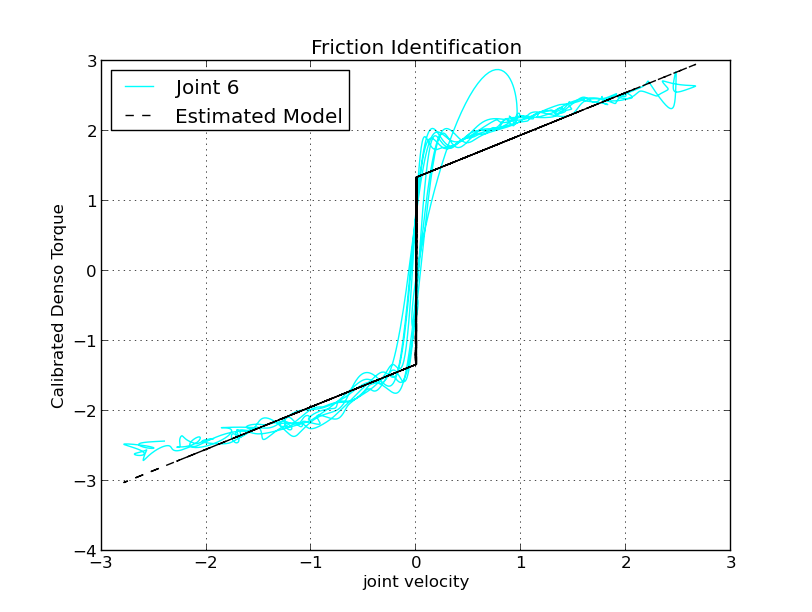
\includegraphics[width = \textwidth ]{A_7_6}
    \caption{Sixth Joint}
  \end{subfigure}
\end{figure}

\section*{Contact Force Estimation Algorithm}
\begin{figure}[H]
  \caption{Contact Force Estimation Algorithm}  
  \label{fig:algo code}
  \begin{subfigure}[t]{\textwidth}
    \centering
    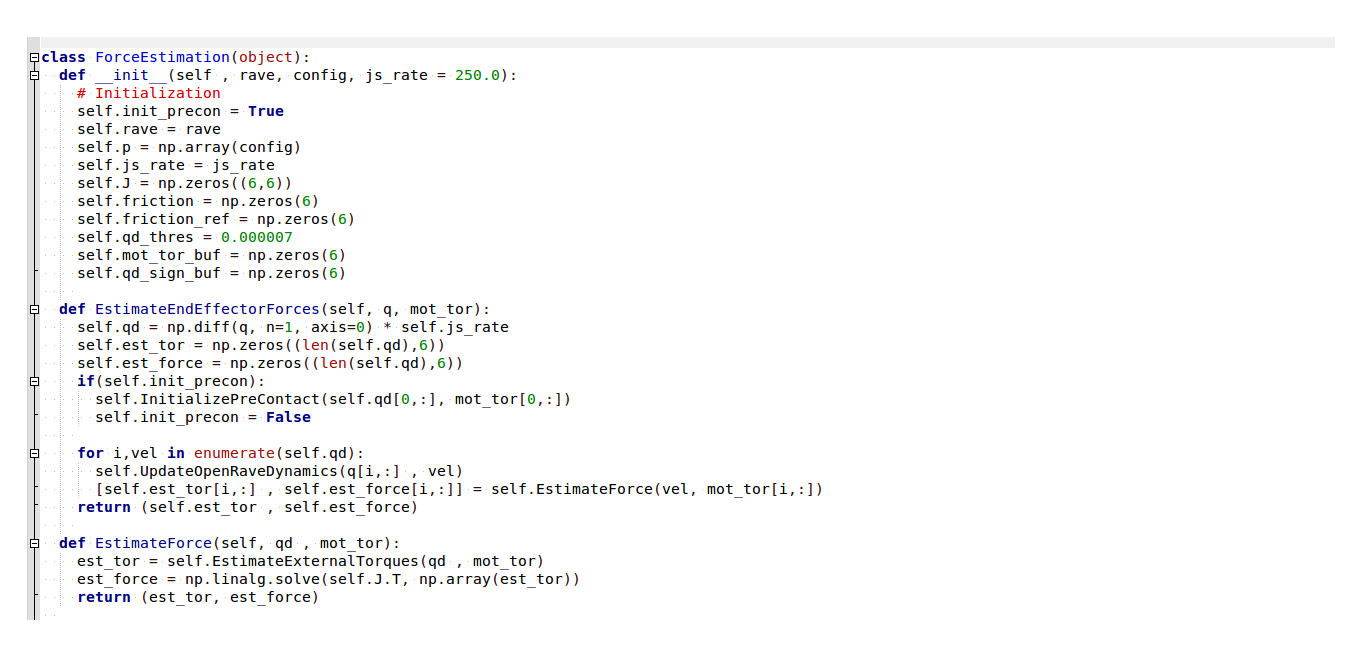
\includegraphics[width = \textwidth ]{A_8_1} 
    \caption{snippet code}
  \end{subfigure}
  \begin{subfigure}[t]{\textwidth}
    \centering
    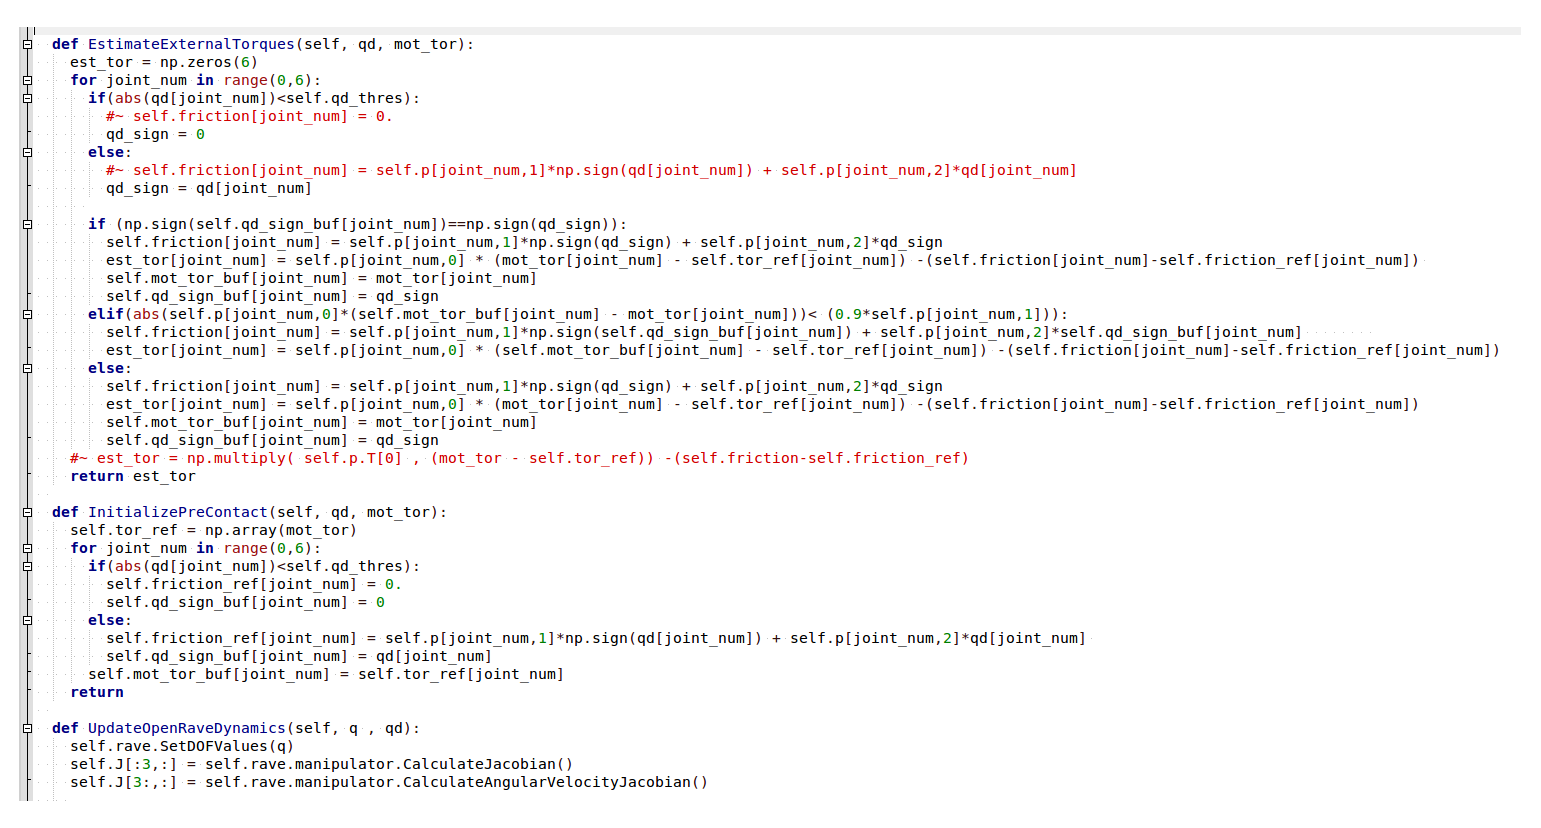
\includegraphics[width = \textwidth ]{A_8_2}
    \caption{snippet code (continued)}
  \end{subfigure}
\end{figure}

\section*{Verification of Two-Stage Results}
\begin{figure}[H]
  \caption{Static contact force}
  \label{fig:appendix static contact}  
  \begin{subfigure}[t]{0.5\textwidth}
    \centering
    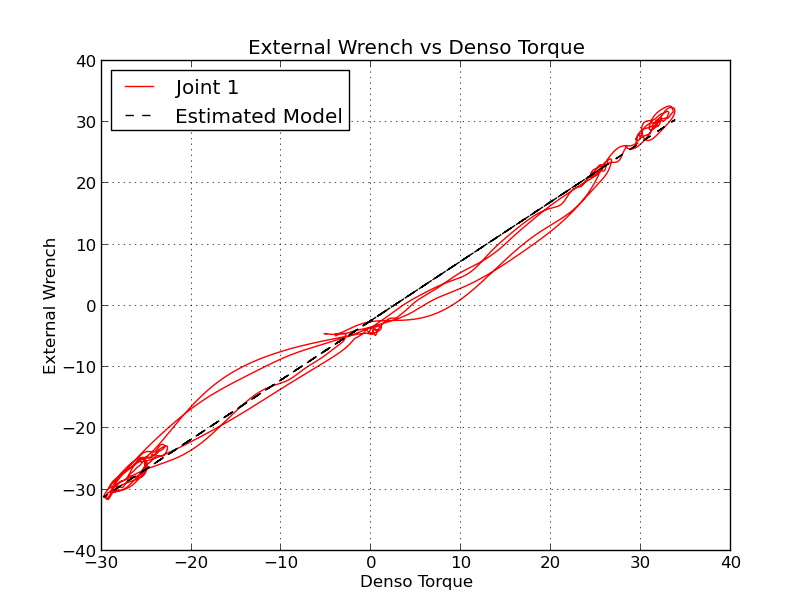
\includegraphics[width = \textwidth ]{A_6_1} 
    \caption{Force x}
  \end{subfigure}
  \begin{subfigure}[t]{0.5\textwidth}
    \centering
    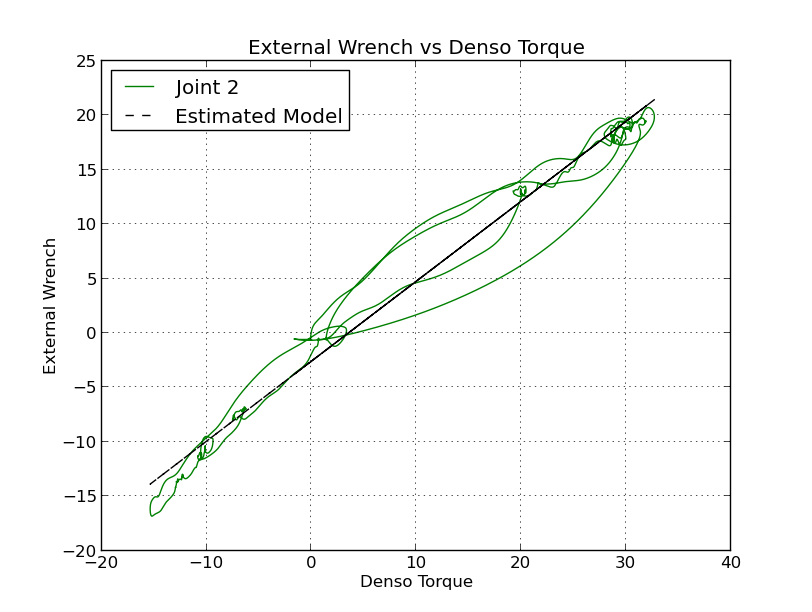
\includegraphics[width = \textwidth ]{A_6_2}
    \caption{Force y}
  \end{subfigure}
  \begin{subfigure}[t]{0.5\textwidth}
    \centering
    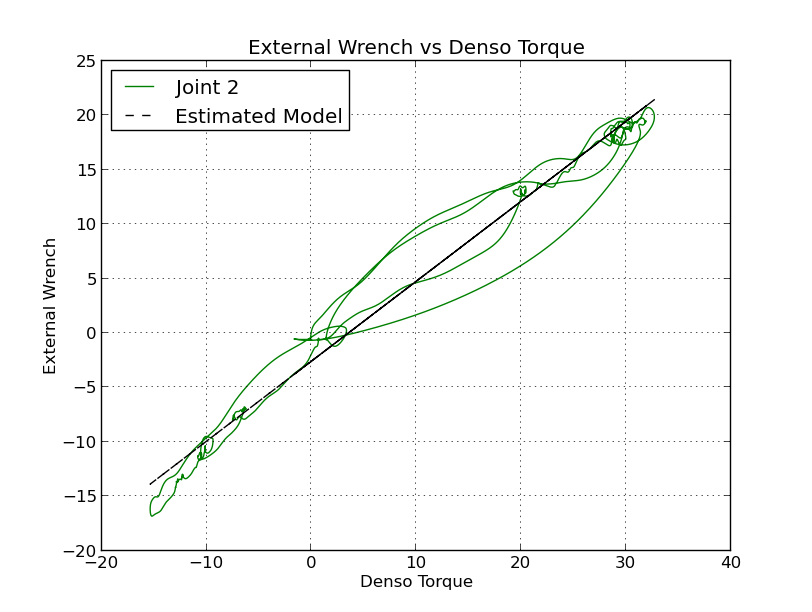
\includegraphics[width = \textwidth ]{A_6_2}
    \caption{Force z}
  \end{subfigure}
  \begin{subfigure}[t]{0.5\textwidth}
    \centering
    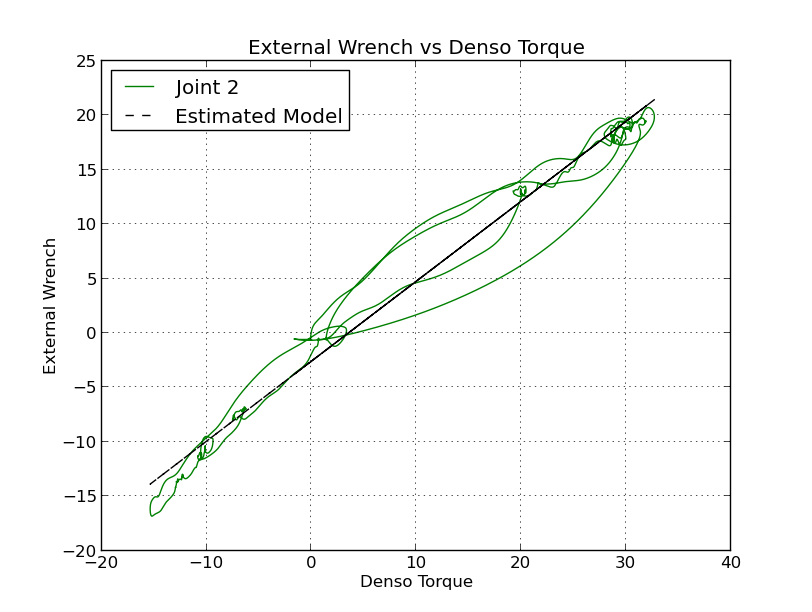
\includegraphics[width = \textwidth ]{A_6_2}
    \caption{Torque x}
  \end{subfigure}
  \begin{subfigure}[t]{0.5\textwidth}
    \centering
    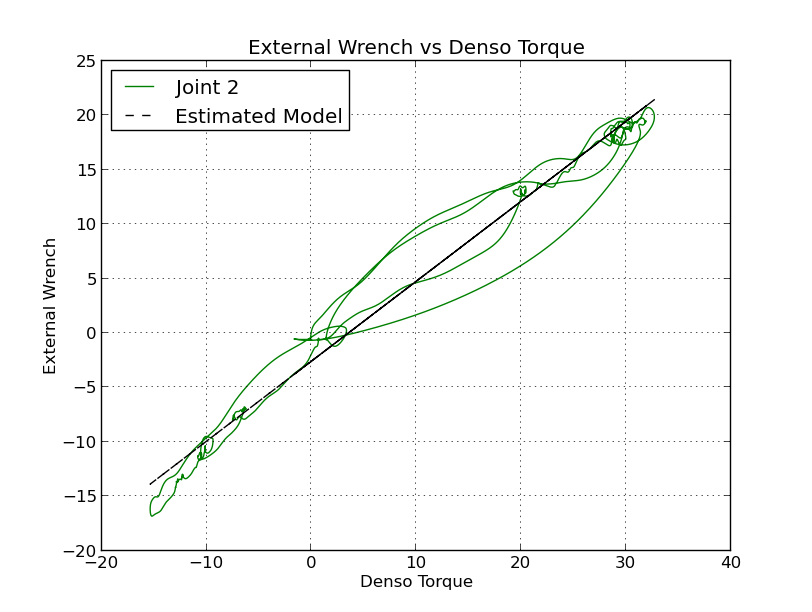
\includegraphics[width = \textwidth ]{A_6_2}
    \caption{Torque y}
  \end{subfigure}
  \begin{subfigure}[t]{0.5\textwidth}
    \centering
    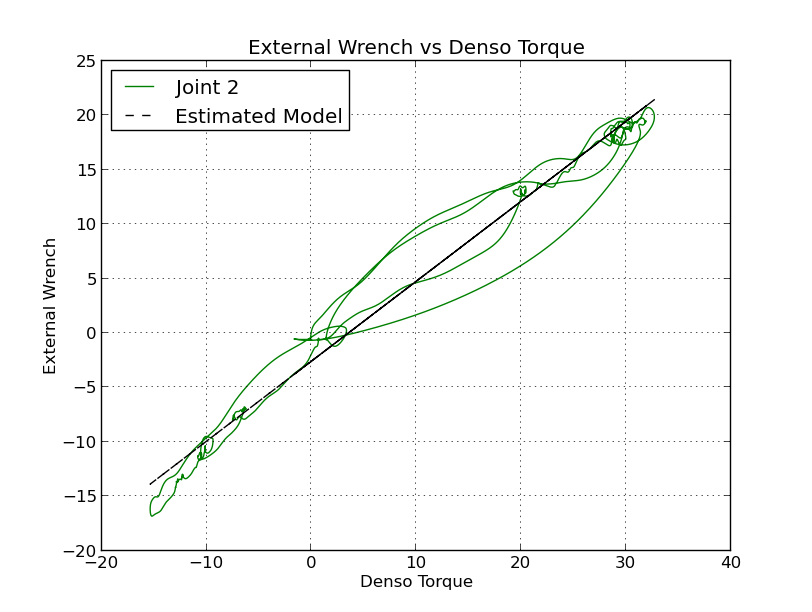
\includegraphics[width = \textwidth ]{A_6_2}
    \caption{Torque z}
  \end{subfigure}
\end{figure}

\begin{figure}[H]
  \caption{Sinusoidal contact force}  
  \begin{subfigure}[t]{0.5\textwidth}
    \centering
    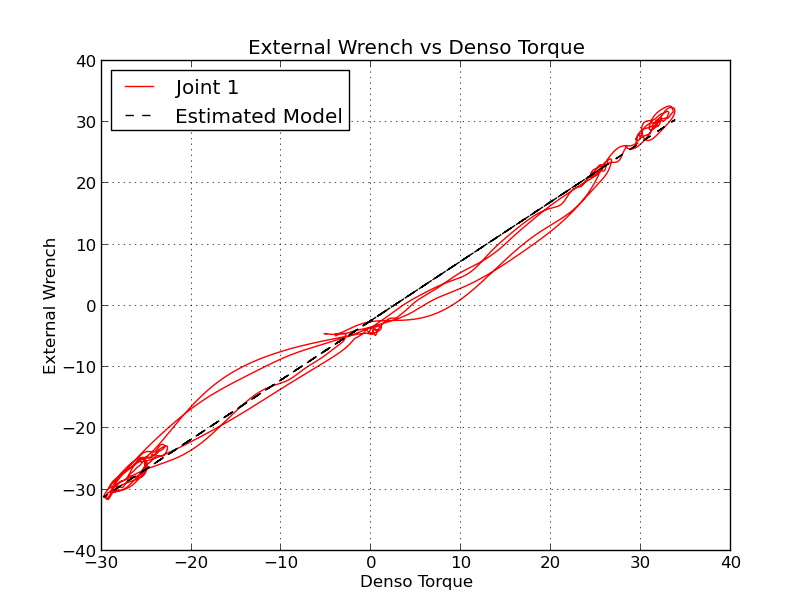
\includegraphics[width = \textwidth ]{A_6_1} 
    \caption{Force x}
  \end{subfigure}
  \begin{subfigure}[t]{0.5\textwidth}
    \centering
    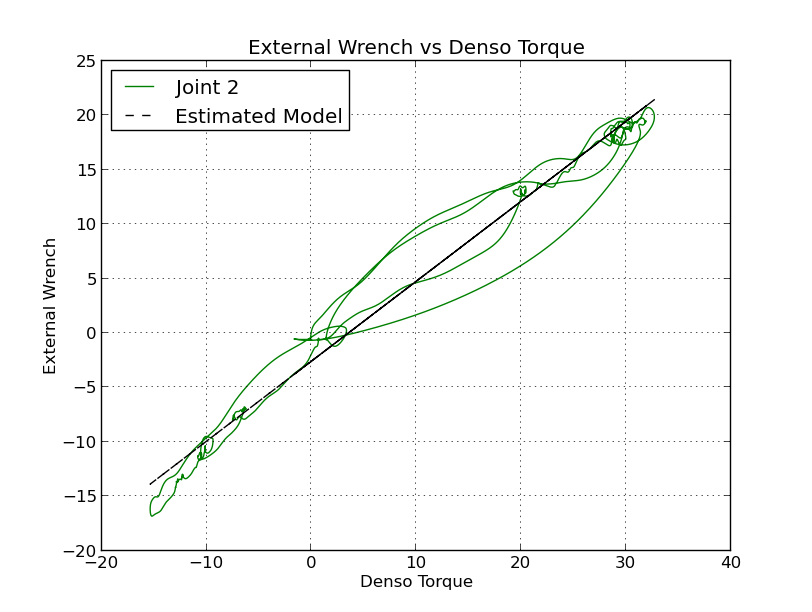
\includegraphics[width = \textwidth ]{A_6_2}
    \caption{Force y}
  \end{subfigure}
  \begin{subfigure}[t]{0.5\textwidth}
    \centering
    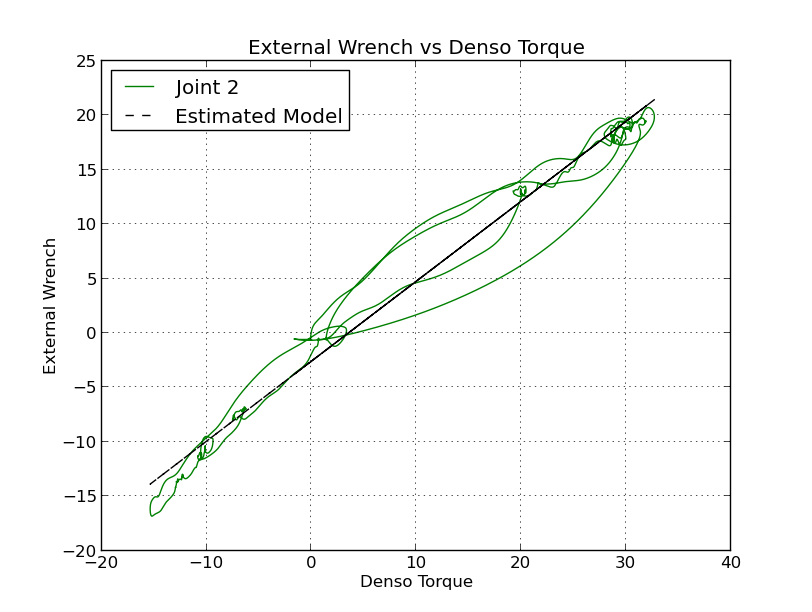
\includegraphics[width = \textwidth ]{A_6_2}
    \caption{Force z}
  \end{subfigure}
  \begin{subfigure}[t]{0.5\textwidth}
    \centering
    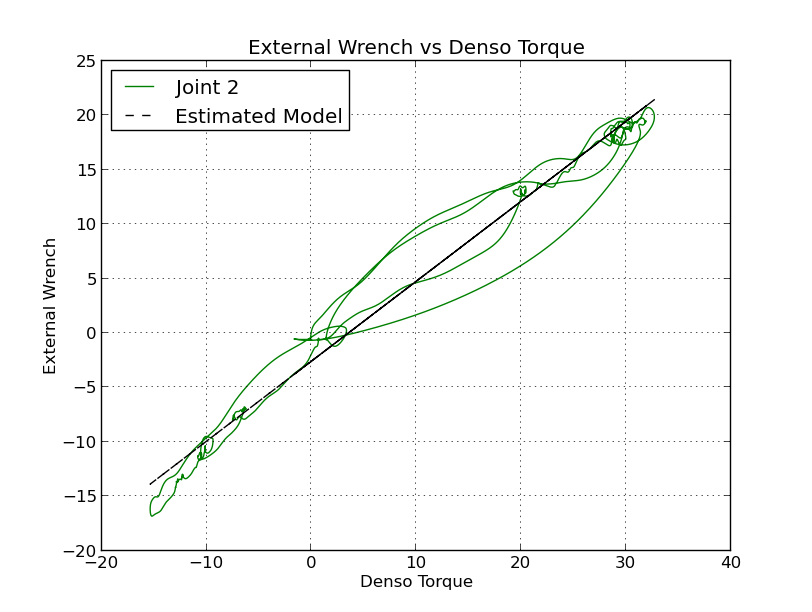
\includegraphics[width = \textwidth ]{A_6_2}
    \caption{Torque x}
  \end{subfigure}
  \begin{subfigure}[t]{0.5\textwidth}
    \centering
    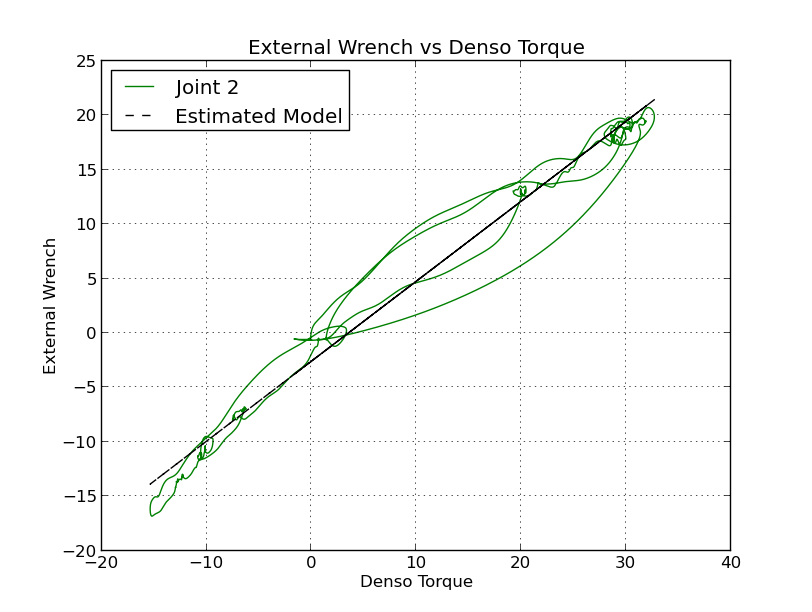
\includegraphics[width = \textwidth ]{A_6_2}
    \caption{Torque y}
  \end{subfigure}
  \begin{subfigure}[t]{0.5\textwidth}
    \centering
    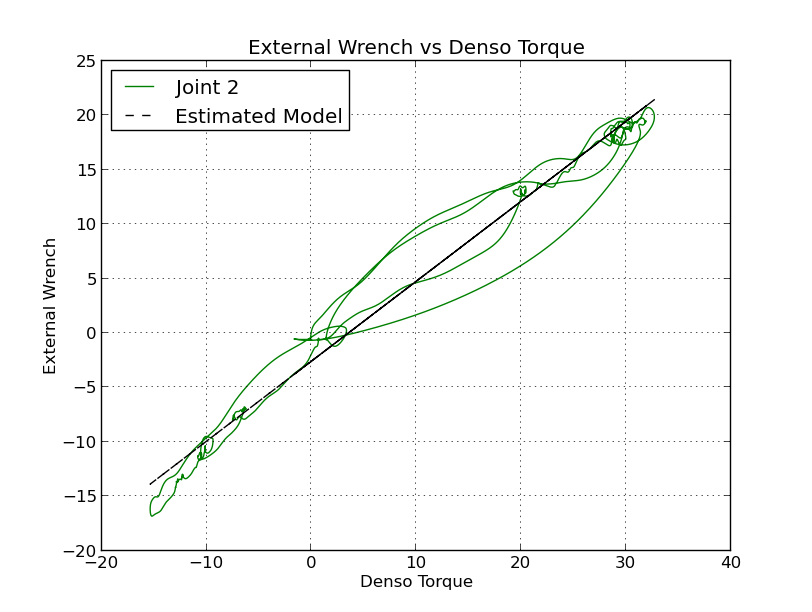
\includegraphics[width = \textwidth ]{A_6_2}
    \caption{Torque z}
  \end{subfigure}
\end{figure}

\begin{figure}[H]
  \caption{Step function contact force} 
  \label{fig:appendix step contact} 
  \begin{subfigure}[t]{0.5\textwidth}
    \centering
    \includegraphics[width = \textwidth ]{A_6_1} 
    \caption{Force x}
  \end{subfigure}
  \begin{subfigure}[t]{0.5\textwidth}
    \centering
    \includegraphics[width = \textwidth ]{A_6_2}
    \caption{Force y}
  \end{subfigure}
  \begin{subfigure}[t]{0.5\textwidth}
    \centering
    \includegraphics[width = \textwidth ]{A_6_2}
    \caption{Force z}
  \end{subfigure}
  \begin{subfigure}[t]{0.5\textwidth}
    \centering
    \includegraphics[width = \textwidth ]{A_6_2}
    \caption{Torque x}
  \end{subfigure}
  \begin{subfigure}[t]{0.5\textwidth}
    \centering
    \includegraphics[width = \textwidth ]{A_6_2}
    \caption{Torque y}
  \end{subfigure}
  \begin{subfigure}[t]{0.5\textwidth}
    \centering
    \includegraphics[width = \textwidth ]{A_6_2}
    \caption{Torque z}
  \end{subfigure}
\end{figure}
